% !TeX spellcheck = en_GB
% !TeX encoding = UTF-8
% !TeX root = ../report.tex

\chapter{Communication}
\label{chp:Communication}

To handle the communication between all devices, a fast and easy to implement data exchange method was required. RIMO, as well as the other manufacturers of our components made use of the standardized industrial application CANOpen. Because CANOpen is based on CAN, we will first describe the CAN bus protocol.

\section{CAN Basics}


CAN stands for Control Area Network and consists of two main layers, namely the physical layer and the data link layer. CAN was developed in 1986 and is used for data exchange between different stations in a network, based on serial communication. Messages are received and transmitted via broadcasting, making every message available for all of the connected stations. 
%importance and pros cons of can

The rise in electronification in many parts of the industry called for simpler and more efficient means of communication. Extensive wiring still resulted in rather limited data exchange. A way out of this was presented by serial bit data exchange and connecting up all electronic control units to a single bus. Depending on the bus length, CAN offers up to 1 Mbit/s of data rate, while remaining robust and reliable, even in a noisy environment.

The physical layer consists of a twisted pair of wires, which can be shielded if required. The value of a bit was determined by the difference in voltage of the two wires. If the voltages are the same, the bit is recessive. If the difference is higher than 0.9 V, the bit is dominant. As both wires are affected by the same electromagnetic disturbances, their difference in voltage will not vary. The data link is therefore immune to electromagnetic disturbances. By twisting the wires, the magnetic field generated will also be reduced significantly.

%graphic of can network
%elaborate on physical layer and simple message, 60 ohm when measured as both ends parallel
%baud rate

To reduce reflections in the data cables with rates higher than 125kbit/s, it is recommended to terminate the ends of the communication lines with termination resistors with 120 Ohm. 

\newpage

Roughly speaking, a CAN message or frame is made up of an identifier(ID) and the data (up to 8 bytes). A complete CAN message looks like the following.
%picture and example of can message

\begin{tabular}{|c|c|}
	\hline 
	\textbf{Name} & \textbf{Length in bits} \\ 
	\hline 
	SOF & 1 \\ 
	\hline 
	ID & 11 \\ 
	\hline 
	RTR & 1 \\ 
	\hline 
	ID extension & 1 \\ 
	\hline 
	Reserved bit & 1 \\ 
	\hline 
	DLC & 4 \\ 
	\hline 
	Data & 0-64 \\ 
	\hline 
	CRC & 15 \\ 
	\hline 
	CRC delimiter & 1 \\ 
	\hline 
	ACK slot & 1 \\ 
	\hline 
	ACK delimiter & 1 \\ 
	\hline 
	EOF & 7 \\ 
	\hline 
\end{tabular} 

SOF describes the start of the frame, followed by the identifier. The role of the identifier bit is important, as it handles bus management and represents the message priority. The remote transmit request (RTR) must be dominant for data frames and recessive for remote request frames. A remote frame is used to request data transmission from a node. The ID extension and reserved bit are dominant for base frames. The data length code (DLC) informs the receiver about the size of the data in bytes, followed by the actual data. The cyclic redundancy check is used for error detection, with the recessive CRC delimiter coming right after. The acknowledgement slot is used to confirm the message by the receiver by using a dominant bit and the transmitter sends a recessive bit. Again, a recessive delimiter ends the acknowledgement slot. The last 7 bits describe the end of the CAN frame.

\newpage

\section{CANOpen}

CANOpen is a higher-layer protocol based on the aforementioned CAN. In the following, we will provide information on the project-relevant aspects of CANOpen.
All real-time data is exchanged via process data objects (PDO). The adress of each individual PDO can be found in a standardized table by CAN in Automation (CiA). PDO's contain data from a single or different objects from the object dictionary. This maps each bit of the data section of a PDO to a certain object.

To change PDO mapping or customise other parameters stored in the object dictionary, service data objects (SDO) are used. These however do not transmit and receive real-time data, but are only used for service purposes. They usually contain the index, subindex and the new value of the respective object.

PDO as well as SDO communication is split into receive and transmit messages.
 For PDO communication the receive PDO contains the desired command for a node and the Transmit PDO is composed of the actual state or other valuable information measured on node itself.

In SDO communication a receive-SDO is either used to change a value in the object dictionary or to request the contents of an entry in the object dictionary. The receive-SDO is always answered by a corresponding transmit-PDO either acknoledging a change in the object dictionary or serving the requested data.

So for example, the mapping of the ACD's RPDO1 looks like the following.

\begin{tabular}{|c|c|c|c|}
	\hline 
	Name & Index & Subindex & Bit \\ 
	\hline 
	&  &  &  \\ 
	\hline 
	Command Word & 0x2000 & 1 & 16 \\ 
	\hline 
	Command Speed & 0x2000 & 2 & 16 \\ 
	\hline 
	Command Acceleration & 0x2000 & 5 & 8 \\ 
	\hline 
	Command Deceleration & 0x2000 & 6 & 8 \\ 
	\hline 
\end{tabular} 
\\
\\
\textit{Table 1, RPDO1 of the ACD 4805}

So in order to set a desired speed on the right (Node 6) motor controller of around 900 rpm, the following message had to be sent.

\begin{tabular}{|c|c|c|c|c|c|c|}
	\hline 
	CAN-ID & \multicolumn{6}{c|}{DATA} \\ 
	\hline 
	0x206 & 09 & 00 & 84 & 03 & 00 & 00 \\ 
	\hline 
\end{tabular} 

Take note that to translate the desired target input into a bytewise message
the little endian rule is most often utilized and the hex format is used to display the contents of each byte. According to the little endian rule the byte containing the higher bit values comes second in transmission. 
The Command speed of the message above is split into two hex numbers yielding the underlying number 384h.

\newpage

Each CAN device has a personal node, ranging from 1 to 127. This ensures that every message reaches it's corresponding device.
% example of pdo can message


% example of sdo can message
%keywords
%transmission type, can id, sdo, pdo, NMT
There are various transmission types avaible in CANOpen for PDOs. Some are manufacturer specific, therefore only the types relevant for our project will shortly be described.

\begin{itemize}

\item Transmission type 1-240 (cyclic synchronous)
\begin{itemize}
	\item This transmission type relies on sync messages. After every nth sync messages, the PDO transmits it's data. So for example, if the transmission type is 6, the PDO will send after every 6th sync message.
	
	For the Linmot, we used the transmission type one. So in order to gain information about the motor, we had to send sync messages.
	
\end{itemize}

\item {Transmission type 254/255 (asynchronous)}
\begin{itemize}
	\item These transmission types are event-triggered, where the event is manufacturer specific for 254 and for 255 defined in the CANOpen device profile.
	
	For the ACD 4805, tranmission type 254 was listed as unpack the data immediately. This was the setting used in the ACD and in the Mircoautobox.
	
	For the LinMot, transmission type 254 was event triggered, with an adjustable internal timer which triggers the event.
\end{itemize}

\end{itemize}


%busheavy, buslight, busoff, correct baudrate etc.



The standard table of CAN-Id's can be found below.

\begin{tabular}{|c|c|c|}
	\hline 
	\textbf{COB} & \textbf{Function Code} & \textbf{Resulting CAN-ID} \\ 
	\hline 
	NMT &  0000$_{b}$  & $0 (000_{h})$  \\ 
	\hline 
	CODE & $0001_{b}$ &  $128 (080_{h})$\\ 
	\hline 
	TIME & $0010_{b}$ &  $256 (100_{h})$\\ 
	\hline 
	EMCY & $0001_{b}$ &   $129 (081_{h}) $–  255 (0FF$_{h})$ \\ 
	\hline 
	PDO1(tx) & $0011_{b}$ &  $385 (181_{h}) $ – 511 (1FF$_{h})$\\ 
	\hline 
	PDO1(rx) & $0100_{b}$ &  $513 (201_{h}) $ –  639 (27F$_{h})$\\ 
	\hline 
	PDO2(tx) & $0101_{b}$ &  $641 (281_{h}) $ –  767 (2FF$_{h})$\\ 
	\hline 
	PDO2(rx) & $0110_{b}$ &  $769 (301_{h})$  –  895 (37F$_{h})$\\ 
	\hline 
	PDO3(tx) & $0111_{b}$ &  $897 (381_{h}) $ – 1023 (3FF$_{h})$\\ 
	\hline 
	PDO3(rx) & $1000_{b}$ &  $1025 (401_{h}) $ –  1151 (47F$_{h})$\\ 
	\hline 
	PDO4(tx) & $1001_{b}$ &  $1153 (481_{h}) $ –  1279 (4FF$_{h})$\\ 
	\hline 
	PDO4(rx) & $1010_{b}$ & $1281 (501_{h}) $ –  1407 (57F$_{h})$\\ 
	\hline 
	SDO(tx) & $1011_{b}$ & $ 1409 (581_{h}) $ –  1535 (5FF$_{h})$\\ 
	\hline 
	SDO(rx) & $1100_{b}$ & $1537 (601_{h}) $ –  1663 (67F$_{h})$\\ 
	\hline 
	NMT error control &$ 1110_{b} $& $ 1793 (701_{h}) $ –  1919 (77F$_{h})$\\ 
	\hline 
\end{tabular} 
\\
\\
\textit{Table 2, COBs and there corresponding CAN-IDs}
%adjust table number







%brief explaination on additional features, their advantages and how they benefited us.


\section{Matlab Model}

In the following passage, some of the most important components of the matlab model will be explained. The matlab model is the underlying software basis for the C code running on the Microautobox handling the CAN bus and all communication on it.

The physical layer of CAN has been set up in the multimessage controllersetup block. The baudrate has been set to 250 Kb/s. The module together with the board number determine the pins for the CAN connection. Moreover, Various status messages of the CAN bus can be read out from this block.

The CANOpen general setup block generates a matlab block for each node on the CAN bus, sets the transmission type for each message and determines the sync interval for the network. The Sync interval has been set to 2ms and the transmission type has been defined as cyclic synchronous for all nodes. The heartbeat message and nodeguarding have been turned off in this first prototype.

The blocks generated by the general setup block allow for numerous inputs and outputs. Some of the most important functionalities are the following:

\begin{description}
	\item[Sync Block]
	The sync block generates the sync block according to the interval defined earlier. The input turns the sync message on or off.
	\item[Reset] 
	By feeding a rising edge into this input a node can be resetted. 
	\item[NMT Timeout]
	The time the nodes have to restart after a reset. If a node takes longer to restart than stated by this expression an error will occur.
	\item[SDO Trigger]
	To send a SDO message a rising edge must be fed into this port.  
	\item[SDO W and RXPDO Data] 
	The data for PDO respectively SDO transmission can be led into this input. The data is composed of vectors of data type uint8, each integer representing on byte.The data will be transmitted with the corrresponding identifier by default.
	\item[SDO R and TXPDO data] 
	The response to a SDO message and the cyclic transmission of the TXPDO can be read out here. The bytes of all TXPDO are encapsuled in one vector.
	
\end{description}

The following picture shows the multimessage controllersetup block and the node blocks created by the CANOpen general setup block.
%Bilder
\begin{figure}[h]
	\centering
	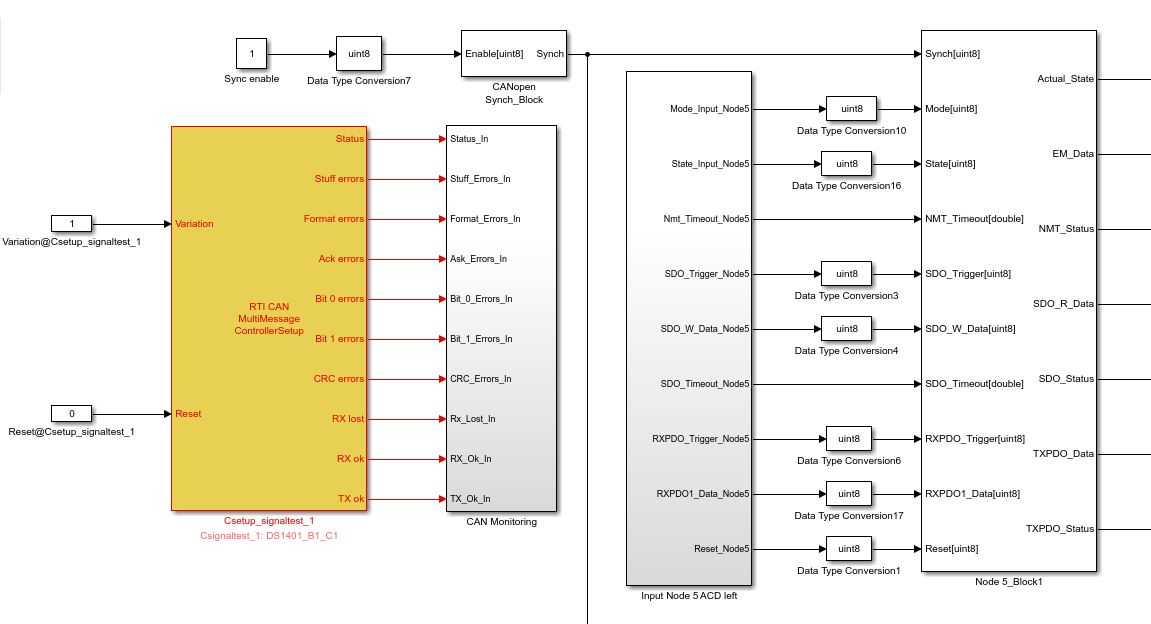
\includegraphics[width=0.7\linewidth]{pictures_figures/Used/Picture_Matlab}
	\caption{}
	\label{fig:picturematlab}
\end{figure}



\subsection{Analogue Digital Converter}

To check the voltage of the 12 V battery mounted in the front, we used dSpace's ADC block. The module number 1 and the channel number 1 were used. Because the Microautbox's voltage input range is 0 - 5V, a voltage divider was used. The output of the ADC is between 0 and 1. The voltage input ranges from 0 to ~4.3 V, therefore the maximum output of the ADC is around 0.86. So in order to get the proper scaling, the ADC output gain needs to be around 13.95. 

An additional digital output and input (Microautobox) were utilized to turn on a warning lamp in case of critical error and display the state of the emergency switch. 